\chapter{Problema de Kepler Newtoniano}\label{app:Kepler}

Aqu'i reproduciremos el an'alisis newtoniano de las 'orbitas de un sistema binario, modelado como dos masas puntuales $m_1$ y $m_2$, movi'endose bajo la acci'on de su atracci'on mutua. Si $\vec{x}_1$ y $\vec{x}_2$ son las coordenadas de $m_1$ y $m_2$ respecto a un SRI, respectivamente, entonces las ecuaciones de movimiento correspondientes son:
\begin{equation}
\ddot{\vec{x}}_1=-Gm_2\frac{(\vec{x}_1-\vec{x}_2)}{|\vec{x}_1-\vec{x}_2|^3} ,\label{acel1}
\end{equation}
\begin{equation}
\ddot{\vec{x}}_2=-Gm_1\frac{(\vec{x}_2-\vec{x}_1)}{|\vec{x}_1-\vec{x}_2|^3} .\label{acel2}
\end{equation}
Es conveniente definir la coordenada del \textit{centro de masa} $\vec{x}_{\rm cm}$ por
\begin{equation}
\vec{x}_{\rm cm}:=\frac{m_1\vec{x}_1+m_2\vec{x}_2}{M}, \qquad M:=m_1+m_2.
\end{equation}
Es directo comprobar a partir de (\ref{acel1}) y (\ref{acel2}) que
\begin{equation}
\ddot{\vec{x}}_{\rm cm}=\vec{0}.
\end{equation}
Por lo tanto, la coordenada del centro de masa se mueve a velocidad constante. Esto permite simplificar el problema describiendo el movimiento desde el SRI en el que el centro de masa del sistema est'a en reposo y ubicado en el origen\footnote{M'as generalmente, es posible \textit{separar} el movimiento en el movimiento del centro de masa y el movimiento relativo}, es decir,
\begin{equation}
\vec{x}_{\rm cm}\stackrel{!}{=}\vec{0}. \label{cm}
\end{equation}
La condici'on (\ref{cm}) implica que, en el \textit{SRI del centro de masa} las coordenadas de $m_1$ y $m_2$ est'an relacionadas por
\begin{equation}
\vec{x}_2=-\frac{m_1}{m_2}\vec{x}_1. \label{x2f1}
\end{equation}
Definiendo adem'as la \textit{coordenada relativa}
\begin{equation}
\vec{r}:=\vec{x}_2-\vec{x}_1,
\end{equation}
podemos escribir, usando (\ref{x2f1}),
\begin{equation}\label{x12fr}
\vec{x}_1=-\frac{m_2}{M}\vec{r}, \qquad \vec{x}_2=\frac{m_1}{M}\vec{r}.
\end{equation}
Usando estas relaciones podemos transformar las ecuaciones de movimiento (\ref{acel1}) y (\ref{acel2}) en ecuaciones para la coordenada relativa:
\begin{equation}
\ddot{\vec{r}}=-GM\frac{\hat{r}}{r^2} .\label{acelr}
\end{equation}
Por otro lado, la energ'ia total del sistema,
\begin{equation}
E=\frac{1}{2}m_1\vec{v}_1^2+\frac{1}{2}m_2\vec{v}_2^2-\frac{Gm_1m_2}{|\vec{x}_1-\vec{x}_2|},
\end{equation}
y el momentum angular total respecto al origen,
\begin{equation}
\vec{L}=m_1\vec{x}_1\times\vec{v}_1+m_2\vec{x}_2\times\vec{v}_2,
\end{equation}
pueden reescribirse en t'erminos de la coordenada relativa, resultando
\begin{equation}\label{Er}
E=\frac{1}{2}\mu \vec{v}^2-\frac{G\mu M}{r},
\end{equation}
\begin{equation}\label{Lr}
\vec{L}=\mu\,\vec{r}\times\vec{v},
\end{equation}
donde $\vec{v}:=\dot{\vec{r}}$ y $\mu:=m_1m_2/M$ es llamada la \textit{masa reducida} del sistema.

Los resultados (\ref{acelr}), (\ref{Er}) y (\ref{Lr}) muestran que el movimiento relativo es equivalente al de un cuerpo de masa $\mu$ movi'endose en el potencial central \textit{fijo} generado por una masa $M$ situada en el origen, $\phi=-GM/r$. Como este potencial es central, el momentum angular total del sistema es constante a lo largo de la trayectoria. Como consecuencia, el movimiento est'a confinado al plano perpendicular a $\vec{L}$ (ecl'iptica). Podemos elegir el eje $z$ normal a este plano, de modo que la trayectoria del planeta satisface $\theta=\pi/2$, y entonces
\begin{align}
x & = r\cos\varphi ,\\
y & = r\sen\varphi ,\\
z & = 0.
\end{align}

Usando $\vec{r}=r\,\hat{r}$ podemos escribir la velocidad y la aceleraci'on como
\begin{align}
\vec{v} & = \dot{r}\,\hat{r}+r\dot{\varphi}\,\hat{\varphi} ,\label{vel1}\\
\vec{a} & = \left(\ddot{r}-r\dot{\varphi}^2\right)\hat{r} +\left(r\ddot{\varphi}+2\dot{r}\dot{\varphi}\right)\hat{\varphi} .\label{acer2}
\end{align}
Reemplazando (\ref{acer2}) en (\ref{acelr}) obtenemos
\begin{eqnarray}
\left(\ddot{r}-r\dot{\varphi}^2\right)\hat{r}+
\left(r\ddot{\varphi}+2\dot{r}\dot{\varphi}\right)\hat{\varphi}
=-\frac{GM}{r^2}\hat{r}.
\end{eqnarray}
De aqu'i, encontramos
\begin{eqnarray}
\ddot{r}-r\dot{\varphi}^2&=&-\frac{GM}{r^2},\label{acer3}\\
r\ddot{\varphi}+2\dot{r}\dot{\varphi}&=&0.\label{acer4}
\end{eqnarray}
Multiplicando la segunda ecuaci\'on por $r$, se encuentra que $r^2\dot{\varphi}$ es constante sobre la trayectoria,
\begin{eqnarray}
0&=&r^2\ddot{\varphi}+2r\dot{r}\dot{\varphi}\\
&=&\frac{d\ }{dt}\left(r^2\dot{\varphi}\right),
\end{eqnarray}
que expresa la conservaci'on del momento angular, ya que
\begin{align}
\vec{L} & = \mu\,\vec{r}\times\vec{v}\\
& = \mu\,r\,\hat{r}\times\left(\dot{r}\hat{r}+r\dot{\varphi}\hat{\varphi}
\right)\\
& = \mu\,r^2\dot{\varphi}\,(\hat{r}\times\hat{\varphi})\\
& = \mu\,r^2\dot{\varphi}\,\hat{z}. \label{Ln}
\end{align}
Otra cantidad conservada sobre la 'orbita es la energ\'ia mec\'anica,
\begin{align}
E&=\frac{1}{2}\mu v^2-\frac{GM\mu}{r} \label{ener1}\\
&=\frac{1}{2}\mu\dot{r}^2+\frac{1}{2}\mu r^2\dot{\varphi}^2-\frac{GM\mu}{r}.\label{ener2}
\end{align}
Despejando $\dot{\varphi}$ de (\ref{Ln}) podemos escribir la energ'ia mec'anica s'olo en t'erminos de la variable $r$ y constantes del movimiento:
\begin{eqnarray}
E=\frac{1}{2}\mu\dot{r}^2+\frac{L^2}{2\mu r^2}-\frac{GM\mu}{r} .\label{ener3}
\end{eqnarray}
Es tradicional definir el potencial efectivo
\begin{equation}
V_{\rm ef}(r):=\frac{L^2}{2\mu r^2}-\frac{GM\mu}{r},
\end{equation}
de modo que (\ref{ener3}) puede ser escrita como la ecuaci'on de conservaci'on de la energ'ia de un movimiento unidimensional:
\begin{equation}
E=\frac{1}{2}\mu\dot{r}^2+V_{\rm ef}(r) . \label{EVef}
\end{equation}
El potencial efectivo $V_{\rm ef}(r)$ posee un cero en
\begin{eqnarray}
r_{\rm c}=\frac{L^2}{2GM\mu^2} ,\label{cero1}
\end{eqnarray}
y adem\'as posee un m\'inimo en
\begin{eqnarray}
r_{\rm min}=\frac{L^2}{GM\mu^2}=2r_{\rm c},\label{rmin}
\end{eqnarray}
tal que
\begin{eqnarray}
V_{\rm ef, min}=-\frac{G^2M^2\mu^3}{2L^2}<0.
\end{eqnarray}
Adem'as, el comportamiento asint'otico del potencial efectivo es
\begin{eqnarray}
\lim_{r\to\infty}V_{\rm ef}(r)&\approx&-\frac{GMm}{r}\rightarrow 0,\\
\lim_{r\to 0}V_{\rm ef}(r)&\approx&\frac{L^2}{2mr^2}\rightarrow +\infty .
\end{eqnarray}
\begin{figure}[H]
 \begin{center}
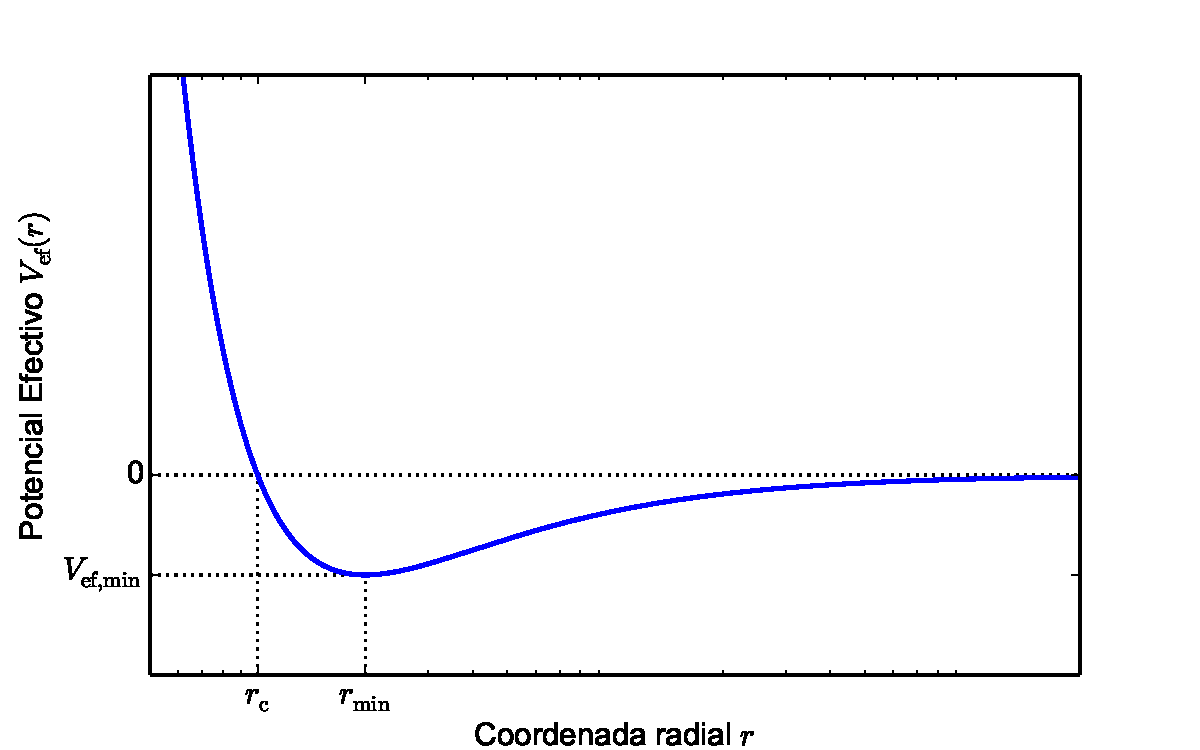
\includegraphics[width=12cm]{fig/fig-potencial-newtoniano.pdf}
\caption{Potencial newtoniano efectivo. Coordenada radial graficada en escala logar'itmica.}
\label{fig:pne}
\end{center}
\end{figure}
As'i, para un valor $L$ dado, tenemos que
\begin{enumerate}
\item Si $E_1>0$, una part'icula proveniente del infinito alcanza un radio
m\'inimo $r_1$, donde $\dot{r}^2=0$, y luego vuelve a infinito.

\item Si $V_{\rm ef, min}<E_2<0$ la trayectoria es ligada, variando la distancia entre dos puntos de retorno $r_2$ y $r_3$, de modo que $r_2<r<r_{3}$.

\item Si $E_{3}=V_{\rm ef, min}$ la part\'icula
describe un movimiento circular de radio dado por (\ref{rmin}). Este caso
corresponde al m\'inimo del potencial, por lo que es un
movimiento estable.

\item Finalmente, no existen trayectorias con $E<V_{\rm ef, min}$ ya que (\ref{EVef}) requiere que $E\ge V_{\rm ef}$.
\end{enumerate}

Determinaremos ahora la forma de la trayectoria, descrita por la dependencia de la coordenada radial $r$ en t'erminos de la coordenada angular $\varphi$. Asumiendo $r=r(\varphi)$ podemos escribir
\begin{eqnarray}
\dot{r}=\frac{dr}{d\varphi}\dot{\varphi}=\frac{L}{\mu r^2}\frac{dr}{d\varphi}.
\end{eqnarray}
Reemplazando esto en (\ref{ener3}) obtenemos
\begin{equation}
\frac{1}{r^4}\left(\frac{dr}{d\varphi}\right)^2=\frac{2\mu E}{L^2}+\frac{2GM\mu^2}{L^2r}-\frac{1}{r^2}.\label{ener4}
\end{equation}
Realizamos ahora el cambio de variable $u:=1/r$, y entonces
\begin{equation}
(u')^2=\frac{2\mu E}{L^2}+\frac{2GM\mu^2}{L^2}\,u-u^{2
},\label{ener5}
\end{equation}
donde $u':=du/d\varphi$. Derivando la expresi\'on anterior se encuentra la ecuaci\'on de
movimiento para $u$ en funci'on de $\varphi$ (para 'orbitas no circulares $u'\neq 0$):
\begin{equation}
u''+u=\frac{GM\mu^2}{L^2}.\label{EC1}
\end{equation}
La integraci\'on de la ecuaci\'on (\ref{EC1}) es directa ya que corresponde a un oscilador arm'onico con un t'ermino forzante constante:
\begin{equation}
u(\varphi)=\frac{GM\mu^2}{L^2}\left(1+e\cos
(\varphi-\varphi_0)\right)\label{CON1}
\end{equation}
donde (luego de reemplazar esta soluci'on en (\ref{ener5}))
\begin{equation}
e=\sqrt{1+\frac{2L^2E}{G^2M^2\mu^3}}, \label{ex}
\end{equation}
es la \textit{excentricidad} de la 'orbita y $\varphi_0$ es una constante de
integraci'on correspondiente a la orientaci\'on inicial relativa al eje
$x$. Si $-G^2M^2\mu^3/2L^2<E<0$ entonces $0<e<1$, y la
c\'onica es una elipse.

El semieje mayor de la 'orbita,
\begin{equation}
a=\frac{1}{2}\left(r_{\rm max}+r_{\rm min}\right),
\end{equation}
puede ser escrito en t'erminos de las constantes del movimiento, a partir de (\ref{CON1}) y (\ref{ex}), ya que
\begin{align}
a & = \frac{1}{2}\left(\frac{1}{u_{\rm min}}+\frac{1}{u_{\rm max}}\right) \\
& = \frac{1}{2}\left(\frac{L^2}{GM\mu^2}\frac{1}{(1+e)}+\frac{L^2}{GM\mu^2}\frac{1}{(1-e)}\right) \\
& = \frac{L^2}{GM\mu^2}\frac{1}{(1-e^2)} \\
& = -\frac{GM\mu}{2E}. \label{aE}
\end{align}
Con esto, podemos escribir la soluci'on (\ref{CON1}) como
\begin{equation}
u(\varphi)=\frac{1}{a(1-e^2)}\left[1+e\cos
(\varphi-\varphi_0)\right],
\end{equation}
o, en t'erminos de la coordenada radial relativa,
\begin{equation}\label{rphi}
\boxed{r(\varphi)=\frac{a(1-e^2)}{1+e\cos(\varphi-\varphi_0)}.}
\end{equation}

La evoluci'on temporal de la 'orbita puede ser determinada impl'icitamente de la forma siguiente. Definamos la variable auxiliar $s$ por
\begin{equation}\label{rs}
\boxed{r=:a(1-e\cos s).}
\end{equation}
A partir de esto podemos, usando (\ref{rphi}), encontrar una relaci'on entre $\varphi$ y $s$ sobre la 'orbita. De esta forma, obtenemos
\begin{equation}\label{phiscos}
\boxed{\cos(\varphi-\varphi_0)=\frac{\cos s -e}{1-e\cos s}, }
\end{equation}
y a partir de aqu'i,
\begin{equation}\label{phissen}
\sen(\varphi-\varphi_0)=\sqrt{1-e^2}\,\frac{\sen s}{1-e\cos s}.
\end{equation}
Derivando (\ref{phiscos}) respecto a $s$ y usando (\ref{phissen}) obtenemos
\begin{equation}
\frac{d\varphi}{ds}=\frac{\sqrt{1-e^2}}{1-e\cos s}.
\end{equation}
Con esto, podemos expresar el momentum angular (\ref{Ln}) en t'erminos de $s$:
\begin{align}
L & = \mu r^2 \frac{d\varphi}{dt} \\
& = \mu r^2 \frac{d\varphi}{ds}\frac{ds}{dt} \\
& = \mu a^2\left(1-e\cos s\right)^2 \frac{d\varphi}{ds}\frac{ds}{dt} \\
& = \mu a^2\sqrt{1-e^2}\left(1-e\cos s\right) \frac{ds}{dt} .
\end{align}
Por lo tanto,
\begin{align}
1-e\cos s & = \frac{L}{\mu a^2\sqrt{1-e^2}} \frac{dt}{ds} \\
& =: \omega_0 \frac{dt}{ds}, \label{dtds}
\end{align}
donde hemos introducido $\omega_0$, con unidades de frecuencia, que satisface (usando (\ref{ex})),
\begin{equation}\label{Kepler3}
\boxed{\omega_0^2=\frac{GM}{a^3}.}
\end{equation}
La relaci'on (\ref{dtds}) puede integrarse directamente respecto a $s$. Eligiendo la condici'on inicial $s=0$ para $t=t_0$ obtenemos
\begin{equation}\label{ts}
\boxed{\omega_0(t-t_0)=s-e\sen s.}
\end{equation}

La expresi'on (\ref{ts}), junto con (\ref{rs}) y (\ref{phiscos}) (y/o (\ref{phissen})) suministra una \textit{soluci'on param'etrica} para la 'orbita.
A partir de (\ref{rphi}) vemos que $r(\varphi)$ es periodica con periodo $\Delta\varphi=2\pi$. Adem'as, de (\ref{rs}) y/o (\ref{phiscos}) vemos que este periodo corresponde a un cambio en $2\pi$ en la variable auxiliar $s$. Finalmente, la relaci'on (\ref{rs}) implica que esta periodicidad corresponde a un intervalo de tiempo
\begin{equation}
T=\frac{2\pi}{\omega_0},
\end{equation}
que es entonces el \textit{periodo orbital}. Con esto (\ref{Kepler3}) implica la \textit{tercera ley de Kepler}.